\tikzset{
	main/.style={black, line width=0.4mm, opacity=1},
	second/.style={gray, opacity=5},
	arrow/.style={-latex, shorten >=1ex, shorten <=1ex, bend angle=45}
}
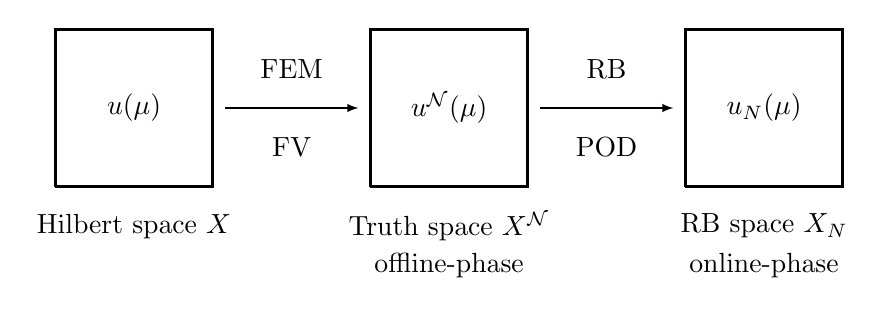
\begin{tikzpicture}
%% Global Matrix
\draw[main] (0,0) -- (2,0) -- (2,2)-- (0,2)-- (0,0);
\draw[main] (4,0) -- (6,0) -- (6,2)-- (4,2)-- (4,0);
\draw[main] (8,0) -- (10,0) -- (10,2)-- (8,2)-- (8,0);


\draw [arrow]  (2,1) to (4,1);
\draw [arrow]  (6,1) to (8,1);


\draw (1,1) node {$u(\mu)$};
\draw (5,1) node {$u^\mathcal{ N }(\mu)$};
\draw (9,1) node {$u_N(\mu)$};

\draw (3,1.5) node {FEM};
\draw (3,.5) node {FV};

\draw (7,1.5) node {RB};
\draw (7,.5) node {POD};

\draw (1,-.5) node {Hilbert space $\mathbb{X}$};
\draw (5,-.5) node {Truth space $\mathbb{X}^\mathcal{ N }$};
\draw (5,-1) node {offline-phase};
\draw (9,-.5) node {RB space $\mathbb{X}_N$};
\draw (9,-1) node {online-phase};


\end{tikzpicture}